\documentclass[a4paper,12pt]{book}

% Paquetes necesarios
\usepackage[utf8]{inputenc}   % Codificación de caracteres
\usepackage[spanish]{babel}   % Idioma español
\usepackage[T1]{fontenc}      % Codificación de fuentes
\usepackage{amsmath, amssymb} % Símbolos matemáticos
\usepackage{graphicx}         % Inclusión de gráficos
\usepackage{cite}             % Gestión de citas
\usepackage{hyperref}         % Enlaces y referencias
\usepackage{geometry}         % Configuración de márgenes
\usepackage{fancyhdr}         % Encabezados y pies de página
\usepackage{titlesec}         % Formato de títulos
\usepackage{booktabs}         % Tablas profesionales
\usepackage{caption}          % Personalización de leyendas
\usepackage{enumitem}         % Personalización de listas
\usepackage{float}
\usepackage{tcolorbox}
\usepackage[table]{xcolor} % Paquete para colores en tablas
\usepackage{colortbl}       % Complemento para colorear celdas específicas
\usepackage{multirow}       % Combinar celdas en tablas
\usepackage{makecell}       % Combinar celdas en tablas
\usepackage{enumitem}
\usepackage{amsmath}
\usepackage{eurosym}
\usepackage{tikz}
\usepackage{listings}
\usepackage{color}
\usepackage{float}
\usepackage{pdfpages}

% Configuración de márgenes
\geometry{left=3cm, right=3cm, top=2.5cm, bottom=2.5cm}

% Configuración de encabezados y pies de página
% \setlength{\headheight}{14.49998pt}
\pagestyle{fancy}
\fancyhf{}
\fancyhead[L]{Universidad de Granada}
\fancyhead[L]{\nouppercase{\chaptername~\thechapter. \leftmark}}

% \fancyhead[C]{Escuela Técnica Superior de Ingenierías Informática}
\fancyhead[R]{Inteligencia Artificial}
\fancyfoot[L]{\rule[0pt]{\textwidth}{0.2pt}\\Ismael Sallami Moreno}
\fancyfoot[C]{\rule[0pt]{\textwidth}{0.2pt}\\\thepage}
\fancyfoot[R]{\rule[0pt]{\textwidth}{0.2pt}\\\today}
\renewcommand{\sectionmark}[1]{\markboth{#1}{}} % Configura \leftmark para que solo muestre la sección


% Formato de títulos
\titleformat{\section}{\large\bfseries}{\thesection.}{0.5em}{}
\titleformat{\subsection}{\normalsize\bfseries}{\thesubsection.}{0.5em}{}

% Datos del documento
\title{\textbf{Prácticas Inteligencia Artificial}}
\author{
    Ismael Sallami Moreno \\
    \texttt{ism350zsallami@correo.ugr.es}
}
\date{
    \vspace{1cm}
    \begin{tabular}{rl}
        \textbf{Asignatura:} & Inteligencia Artificial \\
        \textbf{Tema:} & Prácticas \\
        \textbf{Fecha:} & \today
    \end{tabular}
}

\begin{document}

% Portada
\begin{titlepage}
    \begin{center}
        % \vspace*{1cm}
        
        % \Huge
        % \textbf{Práctica Contabilidad Financiera II}
        \Huge \textbf{Práctica Inteligencia Artificial} 
        % \vspace{0.5cm}
        % \LARGE
        % \textbf{Ismael Sallami Moreno}\\
        % \LARGE
        % \texttt{ism350zsallami@correo.ugr.es}
        % \LARGE
        % \url{https://github.com/Ismael-Sallami}
        
        % \vfill
        
        % \Large
        % \textbf{Universidad de Granada}
        
        \vspace{0.8cm}
        
        \begin{tikzpicture}[remember picture, overlay]
            \node[opacity=0.2] at (current page.center) {
\includegraphics[width=\paperwidth,height=\paperheight]{portada.png}};
            \node[align=center] at (current page.center) {
                
                \vspace{0.5cm}
                \LARGE \textbf{Ismael Sallami Moreno} \\
                \LARGE \texttt{ism350zsallami@correo.ugr.es} \\
                \LARGE \url{https://ismael-sallami.github.io/} \\
                \LARGE \url{https://elblogdeismael.github.io/} \\
                \vspace{2cm}
                \Large \textbf{Universidad de Granada} \\
                \vspace{0.8cm}
                % \Large \textbf{2025}
            };
        \end{tikzpicture}
        \vfill
        
        \Large
        \textbf{2025}
        
    \end{center}
\end{titlepage}
\newpage


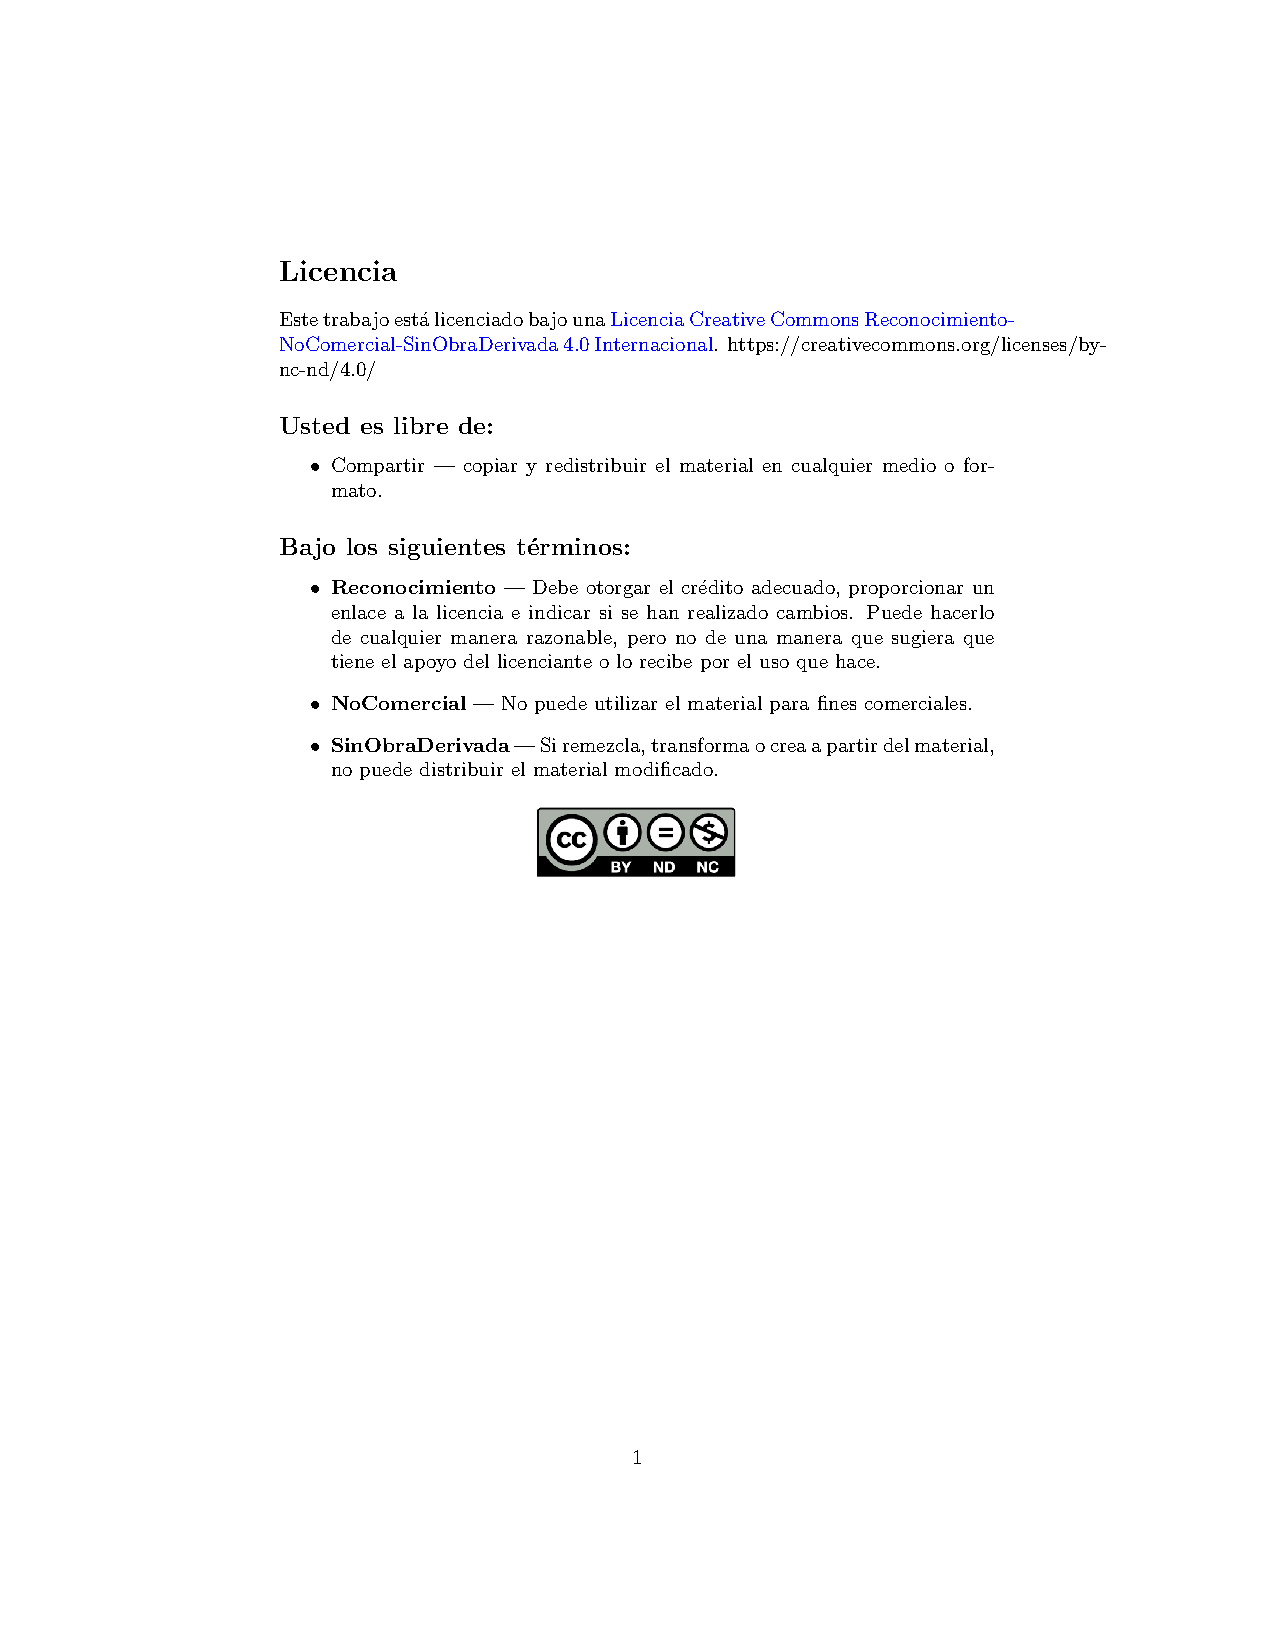
\includepdf[pages=-]{../../../../licencia.pdf}

% Tabla de contenidos
\tableofcontents
\newpage

\chapter{Práctica 1}


\section{Introducción}
% --- IA PR1 ---
\begin{itemize}
    \item \textbf{Agente}: recibe información del entorno, la interpreta y, en base a ello, produce una respuesta.
    \item \textbf{Tipos de agentes}:
    \begin{itemize}
        \item \textbf{Reactivos}: perciben el entorno y toman decisiones concretas basadas en ello. No 'piensan' en un sentido profundo, sino que realizan operaciones con matrices, árboles de decisión y otros métodos para seleccionar una acción. Un ejemplo clásico es el ajedrez.

        Para desarrollar un agente que resuelva un juego como el 8-puzzle, debemos estructurarlo de la siguiente manera:
        \begin{itemize}
            \item Definir el mundo en el que opera, en este caso, un tablero.
            \item Identificar las posibles acciones en cada momento (derecha, izquierda, arriba, abajo) y encontrar un camino óptimo.
        \end{itemize}

        \item \textbf{Deliberativos}: resuelven problemas como el 8-puzzle.  
        
        En este caso, el agente evalúa distintas decisiones posibles y, basándose en ello, encuentra la solución del tablero si existe.  
        Generalmente, esto se resuelve usando estructuras como árboles de búsqueda (por ejemplo, búsqueda en anchura), en los que se analizan los nodos hijos hasta encontrar la solución.  

        Un ejemplo interactivo se puede ver en el siguiente enlace:  
        \url{https://tristanpenman.com/demos/n-puzzle/}, donde la solución correcta aparece resaltada en verde.
    \end{itemize}
    
    \item Una vez diseñado el plan del agente, es importante considerar que, en el mundo real, puede enfrentarse a situaciones para las que no ha sido completamente entrenado.
    \item Algunas características clave a tener en cuenta son: determinismo, observabilidad, dinamismo del entorno, completitud del conocimiento y continuidad.
    \item La IA ha logrado grandes avances en el desarrollo de agentes para mundos cerrados.
\end{itemize}


Para poder enfrentarse a los problemas, la IA debe ser capaz de adaptarse a las situaciones que encuentra en su entorno. Además, debe generalizar soluciones para casos similares basándose en experiencias previas.


En el ámbito del aprendizaje automático, las IA se entrenan para resolver problemas para los cuales no han sido programadas explícitamente. Funcionan sin intervención humana directa. Existen agentes autónomos, que operan sin supervisión, y agentes colaborativos, como los sistemas de IA que conocemos, por ejemplo, ChatGPT y DeepSeek.


También encontramos aplicaciones de autonomía en entornos abiertos, como el desarrollo de agentes en videojuegos como \textit{Minecraft}.


Actualmente, una de las tendencias más populares en IA es el desarrollo de modelos generativos, como ChatGPT. 


Estas inteligencias artificiales han sido entrenadas con enormes conjuntos de datos recopilados de internet. Durante su entrenamiento, se emplean técnicas como la eliminación de partes de un texto, obligando a la IA a predecir y completar la información faltante. Se estima que modelos como los de la familia GPT han sido entrenados con billones de parámetros, lo que representa una capacidad computacional inmensa.


Este tipo de IA presenta tanto fortalezas como debilidades. Por ejemplo, pueden generar código de manera eficiente, pero también pueden cometer errores, lo que limita su fiabilidad en algunos contextos.

\section{Prompts}
En esta sección se nos pedía comprobar que respuesta nos daba ChatGPT a una serie de preguntas. A continuación, se muestran las preguntas y las respuestas obtenidas.

\subsection*{Generar una tabla comparativa entre las ChatGPT, DeepSeek y Gemini}

\begin{table}[H]
    \centering
    \renewcommand{\arraystretch}{1.3}
    \begin{tabular}{|l|p{3cm}|p{3cm}|p{3cm}|}
        \hline
        \textbf{Característica} & \textbf{ChatGPT} & \textbf{DeepSeek} & \textbf{Gemini} \\
        \hline
        \textbf{Desarrollador} & OpenAI & DeepSeek & Google DeepMind \\
        \hline
        \textbf{Modelo de lenguaje} & GPT-4.5 & DeepSeek-R1 & Gemini 1.0 \\
        \hline
        \textbf{Tamaño del modelo} & No especificado & 67 mil millones de parámetros & No especificado \\
        \hline
        \textbf{Entrenamiento} & Datos en múltiples idiomas & Datos en inglés y chino & Datos en múltiples idiomas \\
        \hline
        \textbf{Multimodalidad} & No & No & Sí \\
        \hline
        \textbf{Costo de uso} & Suscripción mensual & Gratuito & Gratuito \\
        \hline
        \textbf{Sesgo y censura} & Respuestas equilibradas & Sesgo pro-Beijing y censura en temas sensibles & Respuestas equilibradas \\
        \hline
        \textbf{Aplicaciones destacadas} & Generación de texto, programación, investigación & Tareas específicas, eficiencia en recursos & Análisis multimodal, integración con servicios de Google \\
        \hline
    \end{tabular}
    \caption{Comparación entre ChatGPT, DeepSeek y Gemini}
    \label{tab:comparacion_modelos}
\end{table}

\subsection{Otros casos}

Se realizaron otra serie de preguntas a ChatGPT y a otras inteligencias artificiales, cosa que no voy a poner aquí porque no aporta nada y no es materia evaluable de examen.

\section{Guía Práctica 1}

\subsection{Ejercicio 1}

En este ejercicio debemos de entrenar una red neuronal para el reconocimiento de sentimientos, si son positivos o negativos:

El primer paso es crear un modelo que sea capaz de clasificar las expresiones que escribimos como positivas o negativas. Puedes imaginarte al modelo como una máquina. Por un lado le metemos un texto y entonces la máquina lo analiza sacando por otro lado el tipo de sentimiento al que pertenece ese texto. El editor de LearningML es la herramienta que usarás para construir este modelo.

\begin{enumerate}
    \item Abre el editor de LearningML. Para ello, dirige tu navegador (Chrome o Firefox) a la dirección \texttt{https://learningml.org/editor}.
    \item Como queremos reconocer textos, pincha en el botón ``Reconocer Textos'', y se abrirá la herramienta con las opciones necesarias para construir un modelo de reconocimiento de texto.
    \item En la sección ``1. Entrenar'', vas a añadir 2 clases (o etiquetas, que también se llaman así), una para cada tipo de conducta. El nombre de estas clases (o etiquetas) serán: \textbf{positivo} y \textbf{negativo}. Para crear una nueva clase pincha en el botón ``Añadir nueva clase de texto''.
    \item Añade a cada clase varios textos que tengan que ver con lo que la clase representa. Te damos algunos ejemplos:

    \begin{itemize}
        \item \textbf{Positivo}
        \begin{itemize}
            \item Si necesita ayuda, dímelo
            \item Puedes contar conmigo
            \item Si no te importa
            \item Si te parece bien
        \end{itemize}
        \item \textbf{Negativo}
        \begin{itemize}
            \item Vete ya hombre
            \item No sirves para nada
            \item No puedo ni verte
        \end{itemize}
    \end{itemize}

    Para añadir nuevos textos a una clase, pincha en el botón ``+'' de esa clase. Fíjate que cada clase tiene su propio botón ``+'' para añadir sus textos.
    \item Muy bien, ya tienes el conjunto de datos de ejemplo. ¡Cuanto más datos añadas, mejor será el resultado! Ahora pincha en el botón ``Aprender a reconocer textos'' de la sección ``2. Aprender''. Asegúrate de que el desplegable ``Lenguaje de los textos'' esté en Español, o escoge el idioma que hayas usado para escribir los textos.
    \item \textbf{IMPORTANTE:} Una vez que pinches en este botón, tu ordenador estará ``aprendiendo'' a partir de los textos que has escrito. Este aprendizaje se hace gracias a un algoritmo que denominamos \textbf{Algoritmo de Machine Learning}. Esto puede tardar un ratito. Sé paciente. Al final de este paso, el algoritmo de Machine Learning ha creado lo que llamamos un \textbf{modelo}. Ese modelo es algo que tú puedes utilizar para que el ordenador reconozca nuevas órdenes parecidas aunque diferentes a las del conjunto de datos de entrenamiento.
    \item Ahora, hay que ver si el modelo que ha construido el algoritmo de Machine Learning funciona bien. Utiliza la caja de texto de la sección ``3. Probar'' para escribir textos que tengan que ver con sentimientos positivos o negativos. Pincha entonces en el botón ``Comprobar'' y observa si lo que dice LearningML coincide con la respuesta correcta.\newline
    \textbf{¡Enhorabuena!} Ya tienes un modelo de inteligencia artificial que reconoce conductas positivas y negativas.
\end{enumerate}

Puede ocurrir que en el paso 6, lo que dice LearningML no coincide con el tipo de conducta correcta. En ese caso, puedes añadir esa frase a la clase que realmente le corresponda y volver a ejecutar el algoritmo de machine learning, es decir, volver a pinchar en el botón ``Aprender a reconocer textos''. Así crearás un nuevo modelo que habrá aprendido esa nueva frase y será más ``potente'', pues es capaz de reconocer correctamente más textos.

También puedes mejorar el análisis de conductas añadiendo una nueva clase para las expresiones que no sean ni de buen rollo ni de malo, es decir, que sean neutras.

El desarrollo de la práctica se encuentre en el apartadao de Prácticas de la asignatura de IA pertenecientes al Tercer Curso, en la web de la \href{https://github.com/ElblogdeIsmael/ElblogdeIsmael.github.io}{asignatura}.





\newpage
% Referencias
\begin{thebibliography}{99}
\bibitem{Referencia1}
Ismael Sallami Moreno, \textbf{Estudiante del Doble Grado en Ingeniería Informática + ADE}, Universidad de Granada, 2025.
% \bibitem{Referencia2}
% Autor(es), \emph{Título del libro}, Editorial, año.

% \bibitem{Referencia3}
% Autor(es), \emph{Título del documento}, Nombre de la Conferencia, páginas, año.
\end{thebibliography}

\end{document}
